\section{Problem}
    A legitimate question would ask why one would need an additional tool to observe their system, observability tools are already plenty and provide useful insights into an application's behaviour.
    
    While they may seem adequate enough to provide a global oversight of applications, they fail to diagnose real time problems like overload, dependent behaviour early enough and in a quick manner. 
    
    The problem we are trying to tackle can be described by the following situation: 

    Imagine an Erlang application instrumented with OpenTelemetry, suddenly, the application starts slowing down, and the execution of a function takes 10 seconds, now, between its start and its end, the user instrumenting the application sees nothing in his dashboard.
    \begin{figure}[H]
        \begin{center}
            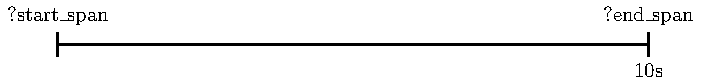
\includegraphics{tikz/start_end.pdf}
        \end{center}
    \end{figure}
    This is a big problem! One would like to know right away if something is wrong with their application. This is where the $\Delta$QSD paradigm and the $\Delta$Q oscilloscope come in handy.
    \begin{figure}[H]
        \begin{center}
            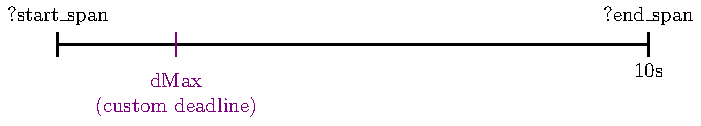
\includegraphics{tikz/start_end_dmax.pdf}
        \end{center}
    \end{figure} 
    By extending $\Delta$QSD notion of early failure one can now right away when the system is overloaded and showing problems, one can know right away when something is wrong, as soon as the maximum delay is hit, this avoids waiting, in this case, 10 seconds to know that something is wrong with your application. \label{timeout}
